\renewcommand{\leveltopI}{-20cm + \leveltop}
\renewcommand{\leveltopII}{-20cm + \leveltopI}
\renewcommand{\leveltopIII}{-20cm + \leveltopII}
\renewcommand{\leveltopIIII}{-20cm + \leveltopIII}
\renewcommand{\leveltopIIIII}{-20cm + \leveltopIIII}
\renewcommand{\leveltopIIIIII}{-20cm + \leveltopIIIII}
\renewcommand{\leveltopIIIIIII}{-20cm + \leveltopIIIIII}
\renewcommand{\leveltopIIIIIIII}{-20cm + \leveltopIIIIIII}
\renewcommand{\leveltopIIIIIIIII}{-20cm + \leveltopIIIIIIII}
\renewcommand{\leveltopIIIIIIIIII}{-20cm + \leveltopIIIIIIIII}
\renewcommand{\leveltopIIIIIIIIIII}{-20cm + \leveltopIIIIIIIIII}
\begin{tikzpicture}[scale=.2, anchor=south]
\begin{scope}[yshift=\leveltopI cm]
\matrix (line1)[column sep=1cm] {
\node[draw=black, rectangle split,  rectangle split parts=4] (sn0xcfd7b0){
\footnotesize{100}
\nodepart{two}
\begin{tikzpicture}[scale=.2]
\node[circle, scale=0.75, fill] (tid0) at (3,1.5){};
\node[circle, scale=0.75, fill] (tid1) at (2.25,3){};
\node[circle, scale=0.75, fill] (tid3) at (2.25,4.5){};
\node[circle, scale=0.75, fill] (tid5) at (2.25,6){};
\node[circle, scale=0.75, fill] (tid7) at (1.5,7.5){};
\node[circle, scale=0.75, fill, red] (tid9) at (0.75,9){};
\node[circle, scale=0.75, fill, red] (tid10) at (2.25,9){};
\draw[](tid7) -- (tid9);
\draw[](tid7) -- (tid10);
\node[circle, scale=0.75, fill, red] (tid8) at (3.75,7.5){};
\draw[](tid5) -- (tid7);
\draw[](tid5) -- (tid8);
\draw[](tid3) -- (tid5);
\draw[](tid1) -- (tid3);
\node[circle, scale=0.75, fill] (tid2) at (5.25,3){};
\node[circle, scale=0.75, fill] (tid4) at (5.25,4.5){};
\node[circle, scale=0.75, fill] (tid6) at (5.25,6){};
\draw[](tid4) -- (tid6);
\draw[](tid2) -- (tid4);
\draw[](tid0) -- (tid1);
\draw[](tid0) -- (tid2);
\end{tikzpicture}
\nodepart{three}
\footnotesize{6.96798}
\nodepart{four}
\footnotesize{$33\:67$}
};
 & 
\\
};
\end{scope}
\begin{scope}[yshift=\leveltopII cm]
\matrix (line2)[column sep=1cm] {
\node[draw=black, rectangle split,  rectangle split parts=4] (sn0xcfffe0){
\footnotesize{33.3333}
\nodepart{two}
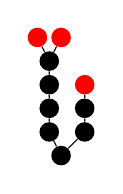
\begin{tikzpicture}[scale=.2]
\node[circle, scale=0.75, fill] (tid0) at (2.25,1.5){};
\node[circle, scale=0.75, fill] (tid1) at (1.5,3){};
\node[circle, scale=0.75, fill] (tid3) at (1.5,4.5){};
\node[circle, scale=0.75, fill] (tid5) at (1.5,6){};
\node[circle, scale=0.75, fill] (tid7) at (1.5,7.5){};
\node[circle, scale=0.75, fill, red] (tid8) at (0.75,9){};
\node[circle, scale=0.75, fill, red] (tid9) at (2.25,9){};
\draw[](tid7) -- (tid8);
\draw[](tid7) -- (tid9);
\draw[](tid5) -- (tid7);
\draw[](tid3) -- (tid5);
\draw[](tid1) -- (tid3);
\node[circle, scale=0.75, fill] (tid2) at (3.75,3){};
\node[circle, scale=0.75, fill] (tid4) at (3.75,4.5){};
\node[circle, scale=0.75, fill, red] (tid6) at (3.75,6){};
\draw[](tid4) -- (tid6);
\draw[](tid2) -- (tid4);
\draw[](tid0) -- (tid1);
\draw[](tid0) -- (tid2);
\end{tikzpicture}
\nodepart{three}
\footnotesize{6.77836}
\nodepart{four}
\footnotesize{$33\:67$}
};
 & 
\node[draw=black, rectangle split,  rectangle split parts=4] (sn0xcfea50){
\footnotesize{66.6667}
\nodepart{two}
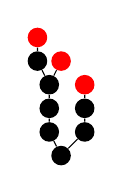
\begin{tikzpicture}[scale=.2]
\node[circle, scale=0.75, fill] (tid0) at (2.25,1.5){};
\node[circle, scale=0.75, fill] (tid1) at (1.5,3){};
\node[circle, scale=0.75, fill] (tid3) at (1.5,4.5){};
\node[circle, scale=0.75, fill] (tid5) at (1.5,6){};
\node[circle, scale=0.75, fill] (tid7) at (0.75,7.5){};
\node[circle, scale=0.75, fill, red] (tid9) at (0.75,9){};
\draw[](tid7) -- (tid9);
\node[circle, scale=0.75, fill, red] (tid8) at (2.25,7.5){};
\draw[](tid5) -- (tid7);
\draw[](tid5) -- (tid8);
\draw[](tid3) -- (tid5);
\draw[](tid1) -- (tid3);
\node[circle, scale=0.75, fill] (tid2) at (3.75,3){};
\node[circle, scale=0.75, fill] (tid4) at (3.75,4.5){};
\node[circle, scale=0.75, fill, red] (tid6) at (3.75,6){};
\draw[](tid4) -- (tid6);
\draw[](tid2) -- (tid4);
\draw[](tid0) -- (tid1);
\draw[](tid0) -- (tid2);
\end{tikzpicture}
\nodepart{three}
\footnotesize{6.56279}
\nodepart{four}
\footnotesize{$33\:33\:33$}
};
 & 
\\
};
\end{scope}
\begin{scope}[yshift=\leveltopIII cm]
\matrix (line3)[column sep=1cm] {
\node[draw=black, rectangle split,  rectangle split parts=4] (sn0xcff620){
\footnotesize{11.1111}
\nodepart{two}
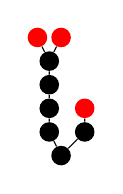
\begin{tikzpicture}[scale=.2]
\node[circle, scale=0.75, fill] (tid0) at (2.25,1.5){};
\node[circle, scale=0.75, fill] (tid1) at (1.5,3){};
\node[circle, scale=0.75, fill] (tid3) at (1.5,4.5){};
\node[circle, scale=0.75, fill] (tid5) at (1.5,6){};
\node[circle, scale=0.75, fill] (tid6) at (1.5,7.5){};
\node[circle, scale=0.75, fill, red] (tid7) at (0.75,9){};
\node[circle, scale=0.75, fill, red] (tid8) at (2.25,9){};
\draw[](tid6) -- (tid7);
\draw[](tid6) -- (tid8);
\draw[](tid5) -- (tid6);
\draw[](tid3) -- (tid5);
\draw[](tid1) -- (tid3);
\node[circle, scale=0.75, fill] (tid2) at (3.75,3){};
\node[circle, scale=0.75, fill, red] (tid4) at (3.75,4.5){};
\draw[](tid2) -- (tid4);
\draw[](tid0) -- (tid1);
\draw[](tid0) -- (tid2);
\end{tikzpicture}
\nodepart{three}
\footnotesize{6.60069}
\nodepart{four}
\footnotesize{$33\:67$}
};
 & 
\node[draw=black, rectangle split,  rectangle split parts=4] (sn0xd05aa0){
\footnotesize{22.2222}
\nodepart{two}
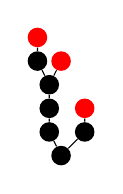
\begin{tikzpicture}[scale=.2]
\node[circle, scale=0.75, fill] (tid0) at (2.25,1.5){};
\node[circle, scale=0.75, fill] (tid1) at (1.5,3){};
\node[circle, scale=0.75, fill] (tid3) at (1.5,4.5){};
\node[circle, scale=0.75, fill] (tid5) at (1.5,6){};
\node[circle, scale=0.75, fill] (tid6) at (0.75,7.5){};
\node[circle, scale=0.75, fill, red] (tid8) at (0.75,9){};
\draw[](tid6) -- (tid8);
\node[circle, scale=0.75, fill, red] (tid7) at (2.25,7.5){};
\draw[](tid5) -- (tid6);
\draw[](tid5) -- (tid7);
\draw[](tid3) -- (tid5);
\draw[](tid1) -- (tid3);
\node[circle, scale=0.75, fill] (tid2) at (3.75,3){};
\node[circle, scale=0.75, fill, red] (tid4) at (3.75,4.5){};
\draw[](tid2) -- (tid4);
\draw[](tid0) -- (tid1);
\draw[](tid0) -- (tid2);
\end{tikzpicture}
\nodepart{three}
\footnotesize{6.36516}
\nodepart{four}
\footnotesize{$33\:33\:33$}
};
 & 
\node[draw=black, rectangle split,  rectangle split parts=4] (sn0xd00870){
\footnotesize{44.4444}
\nodepart{two}
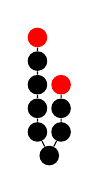
\begin{tikzpicture}[scale=.2]
\node[circle, scale=0.75, fill] (tid0) at (1.5,1.5){};
\node[circle, scale=0.75, fill] (tid1) at (0.75,3){};
\node[circle, scale=0.75, fill] (tid3) at (0.75,4.5){};
\node[circle, scale=0.75, fill] (tid5) at (0.75,6){};
\node[circle, scale=0.75, fill] (tid7) at (0.75,7.5){};
\node[circle, scale=0.75, fill, red] (tid8) at (0.75,9){};
\draw[](tid7) -- (tid8);
\draw[](tid5) -- (tid7);
\draw[](tid3) -- (tid5);
\draw[](tid1) -- (tid3);
\node[circle, scale=0.75, fill] (tid2) at (2.25,3){};
\node[circle, scale=0.75, fill] (tid4) at (2.25,4.5){};
\node[circle, scale=0.75, fill, red] (tid6) at (2.25,6){};
\draw[](tid4) -- (tid6);
\draw[](tid2) -- (tid4);
\draw[](tid0) -- (tid1);
\draw[](tid0) -- (tid2);
\end{tikzpicture}
\nodepart{three}
\footnotesize{6.36719}
\nodepart{four}
\footnotesize{$50\:50$}
};
 & 
\node[draw=black, rectangle split,  rectangle split parts=4] (sn0xd05270){
\footnotesize{22.2222}
\nodepart{two}
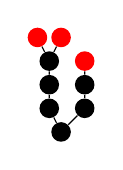
\begin{tikzpicture}[scale=.2]
\node[circle, scale=0.75, fill] (tid0) at (2.25,1.5){};
\node[circle, scale=0.75, fill] (tid1) at (1.5,3){};
\node[circle, scale=0.75, fill] (tid3) at (1.5,4.5){};
\node[circle, scale=0.75, fill] (tid5) at (1.5,6){};
\node[circle, scale=0.75, fill, red] (tid7) at (0.75,7.5){};
\node[circle, scale=0.75, fill, red] (tid8) at (2.25,7.5){};
\draw[](tid5) -- (tid7);
\draw[](tid5) -- (tid8);
\draw[](tid3) -- (tid5);
\draw[](tid1) -- (tid3);
\node[circle, scale=0.75, fill] (tid2) at (3.75,3){};
\node[circle, scale=0.75, fill] (tid4) at (3.75,4.5){};
\node[circle, scale=0.75, fill, red] (tid6) at (3.75,6){};
\draw[](tid4) -- (tid6);
\draw[](tid2) -- (tid4);
\draw[](tid0) -- (tid1);
\draw[](tid0) -- (tid2);
\end{tikzpicture}
\nodepart{three}
\footnotesize{5.95602}
\nodepart{four}
\footnotesize{$67\:33$}
};
 & 
\\
};
\end{scope}
\draw (sn0xcfd7b0.south) -- (sn0xcfffe0.north);
\draw (sn0xcfd7b0.south) -- (sn0xcfea50.north);
\draw (sn0xcfffe0.south) -- (sn0xcff620.north);
\draw (sn0xcfffe0.south) -- (sn0xd00870.north);
\draw (sn0xcfea50.south) -- (sn0xd05aa0.north);
\draw (sn0xcfea50.south) -- (sn0xd00870.north);
\draw (sn0xcfea50.south) -- (sn0xd05270.north);
\end{tikzpicture}

%%% Local Variables:
%%% TeX-master: "thesis/thesis.tex"
%%% End: 
